%----------------------------------------------------------------------------------------
%	PACKAGES AND DOCUMENT CONFIGURATIONS
%----------------------------------------------------------------------------------------
\documentclass[11pt]{article}
\usepackage{amsmath} % Required for some math elements
\usepackage[usenames,dvipsnames]{xcolor}
\usepackage{lipsum} 
\usepackage{cite}
\usepackage{graphicx} % Required for the inclusion of images
\usepackage{algorithmic}
\usepackage{array}
\usepackage{bookmark}
\usepackage{listings}
\usepackage{amssymb}
\usepackage{enumitem}
\usepackage[margin=24mm]{geometry}
\usepackage[caption=false, font=footnotesize]{subfig}
\usepackage{multirow}
\usepackage[active,tightpage]{preview}
\usepackage{hyperref} 



\renewcommand{\PreviewBorder}{1in}
\newcommand{\Newpage}{\end{preview}\begin{preview}}

\newlist{steps}{enumerate}{1}
\setlist[steps, 1]{label = Step \arabic*:}

\hypersetup{ %color attributes of citation, link, etc.
    colorlinks=true,
    linkcolor=blue,
    filecolor=gray,      
    urlcolor=blue,
    citecolor=blue,
}

 
\lstdefinelanguage{VHDL}{
   morekeywords=[1]{
     library,use,all,entity,is,port,in,out,end,architecture,of,
     begin,and,or,Not,downto,ALL
   },
   morekeywords=[2]{
     STD_LOGIC_VECTOR,STD_LOGIC,IEEE,STD_LOGIC_1164,
     NUMERIC_STD,STD_LOGIC_ARITH,STD_LOGIC_UNSIGNED,std_logic_vector,
     std_logic
   },
   morecomment=[l]--
}
\definecolor{keyword}{rgb}{0,0.3,0.7}
\definecolor{STD}{rgb}{0.9,0.0,0.7}
\definecolor{comment}{rgb}{0.0,0.6,0.1}

\lstdefinestyle{vhdl}{
   language     = VHDL,
   basicstyle   = \footnotesize\ttfamily,
   keywordstyle = [1]\color{keyword}\bfseries,
   keywordstyle = [2]\color{STD}\bfseries,
   commentstyle = \color{comment}
   breaklines=true,                % sets automatic line breaking
   tabsize=3		                   % sets default tabsize to 2 spaces
}


\newcommand{\matlab}{\textsc{Matlab }} %very important and totally necessary addition

\newcommand\Item[1][]{%
  \ifx\relax#1\relax  \item \else \item[#1] \fi
  \abovedisplayskip=0pt\abovedisplayshortskip=0pt~\vspace*{-\baselineskip}}
  %----------------------------------------------------------------------------------------
%	DOCUMENT INFORMATION
%----------------------------------------------------------------------------------------
 
\title{ECEN302 : Integrated Digital Electronics \\ Lab 7 Submission : TCL scripts and Packaging IP}
\author{Daniel Eisen : 300447549}
\date{\today}


\begin{document}
\begin{preview}
\maketitle
%----------------------------------------------------------------------------------------
%	DOCUMENT CONTENT
%----------------------------------------------------------------------------------------
\section{Overview}
The use of pre-existing IP blocks in the in HDL design is extremely time saving and in many to most cases is necessary when creating a more complex design with more external dependencies or just utilises a lot of basic reused design blocks. Likewise the IP block system can be made use of to package a preexisting design into a library that can be loaded into the user repository and dropped into block designs or directly instanced without having to redo and grunt work. 
\section{Methodology}
To do this, we initially setup the basic project. Vivado allows for a project to be exported not only as an archive are other larger containers but as set TCL script file and dependency files that can setup project from launch. THis allows for more efficient storage space, can bypass PATH and directory issues upon transfer and just generally can allow for greater flexibility. This is what was used to launch and setup a PWM audio driver project.

The HDL design worked by varying the time step that read through a sine wave LUT to be fed into a PWD generator. This is what effectively changes the frequency and thus pitch of the outputted (filter smoothed) signal/sound.

This project and its 2 HDL modules can be packaged into it own IP block, and exported into a directory that we then imported, add to the user repository and were able to then utilise the generated block as a part of larger design. 

Approaching the design this way enables this relatively simple design to grow easily into a larger and more complex form. This for example is a setup for a larger embedded softcore processor project where the PWM audio IP will be utilised as a peripheral out module to a MicroBlaze uC and driven to play much more complex sequences that can be generated with DIP switches.  


\begin{center}
  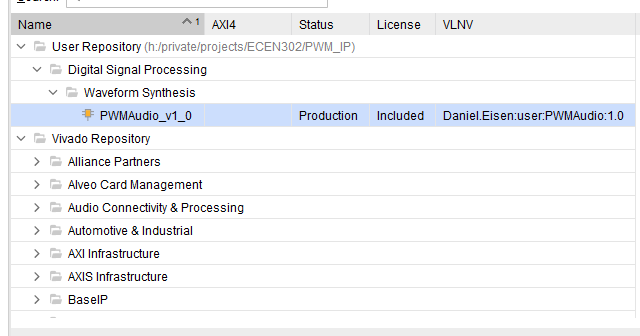
\includegraphics[width=0.5\textwidth]{inc/ip_added.PNG}
\end{center}

\Newpage
\section*{Appendix}
\subsubsection*{PWMAudio}
\lstinputlisting[language=VHDL, style=vhdl]{inc/PWMAudio.vhd}

\Newpage
\subsubsection*{PWMDriver}
\lstinputlisting[language=VHDL, style=vhdl]{inc/PWMDriver.vhd}

\Newpage
\subsubsection*{HDL Wrapper}
\lstinputlisting[language=VHDL, style=vhdl]{inc/design_1_wrapper.vhd}
\end{preview}
\end{document}